\documentclass{parcfd2018}

\usepackage{graphicx}
\usepackage{amsmath}
\usepackage{amsfonts}
\usepackage{amssymb}

\usepackage[
    pdftex,
    pdftitle={Mesnard and Barba, 2018},
    pdfpagemode={UseOutlines},
    bookmarks, bookmarksopen,bookmarksnumbered={True},
    colorlinks, linkcolor={black},citecolor={black},urlcolor={black}
    ]{hyperref}


\title{THREE-DIMENSIONAL FLOW SIMULATIONS OF THE FLYING SNAKE USING MICROSOFT AZURE}

\author{OLIVIER MESNARD$^{*}$ AND LORENA A. BARBA$^{*}$}

\heading{Olivier Mesnard and Lorena A. Barba}

\address{$^{*}$ Department of Mechanical and Aerospace Engineering\\
The George Washington University\\
800 22nd St NW, Washington, DC 20052, United-States\\
e-mail: maeng@gwu.edu, web page: https://www.mae.seas.gwu.edu}

\keywords{Microsoft Azure, CFD, Aerodynamics, Flying snake, PETSc, AmgX, Cloud computing}

\abstract{We ran simulations of the three-dimensional flow around an anatomically correct body section of a flying snake, using our PETSc-based immersed-boundary method code PetIBM on the public cloud platform Microsoft Azure.
The simulations ran on NC24r instances using Azure Batch service and Batch Shipyard, solving the Poisson system on multiple GPU devices with Nvidia AmgX library.}

\begin{document}
%\maketitle

PetIBM,\footnote{\url{https://github.com/barbagroup/PetIBM}} is a PETSc-based open-source code that solves the Navier-Stokes equations with a fully discrete projection method and various immersed-boundary techniques.
Here, we use a decoupled immersed-boundary projection method \cite{Li_et_al_2016}, requiring a Poisson-system solution every time step.
We solve the systems on multiple CUDA-capable GPU devices using the Nvidia AmgX library,\footnote{\url{https://github.com/NVIDIA/AMGX}} interfacing with PETSc via AmgXWrapper \cite{AmgXWrapper}.

We are studying the aerodynamics of \textit{Chrysopelea paradisi}, a species of arboreal snake capable of jumping from tree branches and gliding in the air.
Previous experimental work \cite{Holden_et_al_2014} and two-dimensional simulations \cite{Krishnan_et_al_2014, Mesnard_Barba_2017} found lift enhancement when the glider cross-section forms a $35$-degree angle of attack.
We present new results of the 3D flow around a cylindrical model with anatomically accurate cross-section, at Reynolds number $2000$ and $35$-degree angle of attack, on a  $233$-million-cell structured Cartesian mesh (see Figure 1, bottom).

Thanks to a Microsoft Azure sponsorship, we ran container-based multi-instance tasks for our PetIBM application on NC24r instances (featuring Nvidia K80 GPU devices) with Azure Linux virtual machines and over the Infiniband/RDMA network.
We created the compute pool with Azure Batch, a platform service for running HPC applications in the cloud that relieves the user from manually managing a cluster and task scheduling.
We also used Batch Shipyard,\footnote{\url{https://github.com/Azure/batch-shipyard}} an open-source software to provision and execute container-based tasks on Azure Batch nodes.
The charges for virtual machines, networking, data management, and storage during 2017 added to about \$18,500 of the sponsored account.
On the 233-million-cell mesh, we computed about 75 non-dimensional time units of flow simulation using 6 NC24r nodes for 24 days, at a cost of \$9,511 (with 99\% of the cost incurred by the virtual machines).
We think Microsoft Azure could be a suitable alternative to traditional university HPC clusters to run CFD applications.
Parallel performance compares well (see Figure 1, top).
Based on our experience in the past year, we plan to present our analysis of the cost and other factors that may affect the decision of adopting cloud for CFD.

\begin{figure}[!h]
\centering
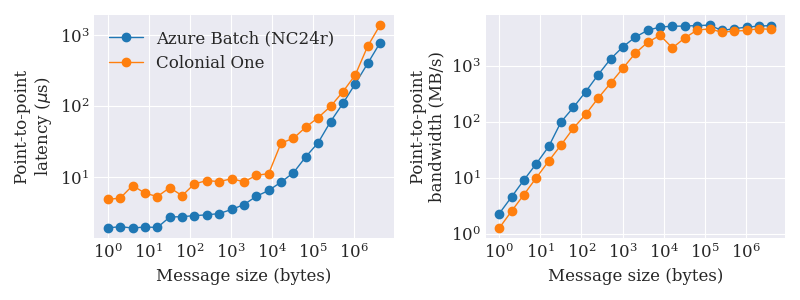
\includegraphics[width=12cm]{figures/latencyBandwidthColonialOneAzure.png}
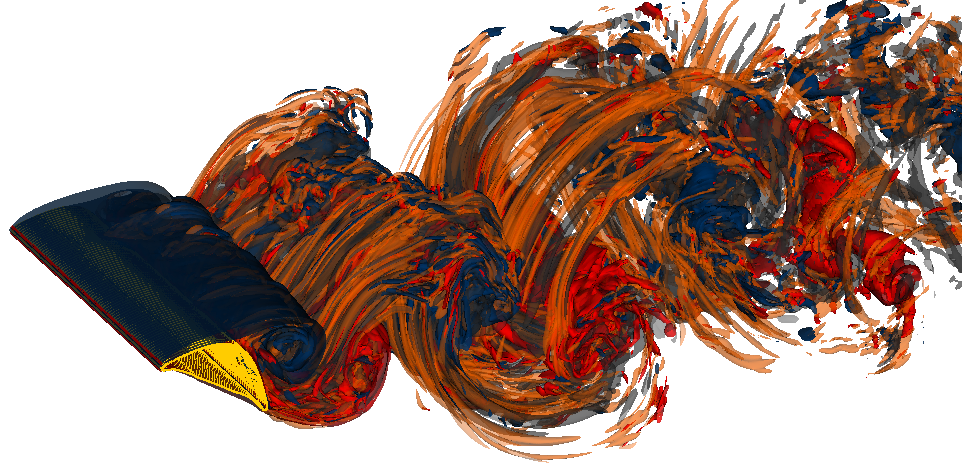
\includegraphics[width=8cm]{figures/wz_wx_wake3d_2k35_meshB_0026.png}
\caption{Top: Point-to-point latency (left) and bandwidth (right) tests performed on a compute pool of two NC24r Azure instances compared with results obtained on our university HPC cluster, Colonial One.
Bottom: Streamwise and spanwise vorticity contours after 141.2 time units of flow simulation for the snake cylinder at Reynolds number $2000$ and angle of attack $35^o$ on a 233-million-cell grid.}
\label{latency_bandwidth_wz_wx}
\end{figure}

\footnotesize
\begin{thebibliography}{99}
\bibitem{Li_et_al_2016}  Li, R.Y., Xie, C.M., Huang, W.X., and Xu, C.X. (2016). \textit{An efficient immersed boundary projection method for flow over complex/moving boundaries}. Computers \& Fluids, 140, 122-135.
\bibitem{AmgXWrapper}  Chuang, P. and Barba, L.A. (2017). \textit{AmgXWrapper: An interface between PETSc and the NVIDIA AmgX library}. Journal of Open Source Software, 2(16), 280, doi:10.21105/joss.00280.
\bibitem{Holden_et_al_2014}  Holden, D., Socha, J.J., Cardwell, N.D., and Vlachos, P.P. (2014). \textit{Aerodynamics of the flying snake Chrysopelea paradisi: how a bluff body cross-sectional shape contributes to gliding performance}. Journal of Experimental Biology, 217(3), 382-394.
\bibitem{Krishnan_et_al_2014} Krishnan, A., Socha, J.J., Vlachos, P.P., and Barba, L.A. (2014). \textit{Lift and wakes of flying snakes}. Physics of Fluids, 26(3), 031901.
\bibitem{Mesnard_Barba_2017}  Mesnard, O. and Barba, L.A. (2017). \textit{Reproducible and Replicable Computational Fluid Dynamics: It's Harder Than You Think}. Computing in Science \& Engineering, 19(4), 44-55.
\end{thebibliography}

\end{document}
